\section{Uniform Sampling}
\label{sec:sampling}

Our goal is to obtain a uniform sample of the Twitter user population. To an
approximation, the sampling frame can be considered all Twitter users, but this
will be refined in Sections~\ref{sec:idsampling}
and~\ref{sec:graphmethods}. Obtaining a sample presents two
challenges: discovering users and picking from them uniformly. In this section, we will discuss what data the Twitter Application Programmer Interfaces (APIs) provide and two sampling methods: one based on generating user \ids~and another based on traversal of Twitter's social network.


\subsection{APIs}

Twitter provides two relevant APIs for programmatic access to Twitter data: the
Streaming API and REST API. The Streaming API provides a continuous random
stream of new tweets. The API does not specify the distribution of users
in this stream (perhaps it could be biased towards users who tweet
frequently or are popular). This makes it suitable for discovering user
\ids~but not for collecting a uniform sample. The REST API provides calls to
GET information about Twitter entities given user identifiers or tweet
identifiers. Like other types of practical surveys, gathering information on
the entire Twitter population is infeasible. This is because the API is rate
limited, restricting a developer to 60-720 requests/hr, depending on the
request type. 

\section{User \id~rejection sampling}
\label{sec:idsampling}

From gathering a collection of Twitter users, we found that the space
of Twitter user \ids~is very dense.  Figure~\ref{fig:id-dist} shows
the distribution of integer user \ids~in this collection. We see that
all \ids~appear to be less than $1e+9$. Given that the rate of larger
\ids~goes down, we assume that few user \ids~lie beyond the range of
integers $[0,1e+9]$. Wikipedia lists Twitter as having about 500
million user accounts, which means that the space of user \ids~is very
dense.  Therefore, we can employ the rejection sampling method used in
\cite{Minas:2009}. For the special case of a uniform target
distribution, the algorithm is simple: uniformly randomly select an
\id~in the range, reject if not a user, and accept if it is a user.
This method was used in \cite{Minas:2009} for Facebook, when user ids
were still 32-bit integers.

\begin{figure}[htb]
\begin{center}
  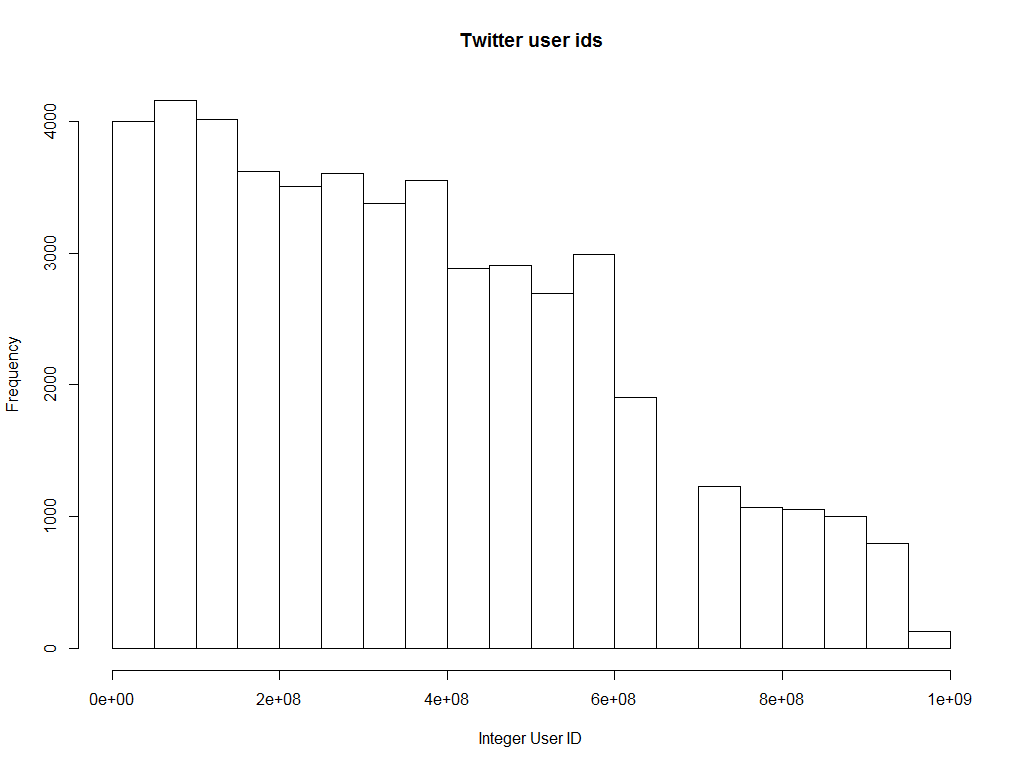
\includegraphics[width=0.8\columnwidth]{figs/user_ids_hist.png}
\end{center}
\caption{Distribution of integer Twitter user IDs from a biased sample of users.}
\label{fig:id-dist}
\end{figure}

  The sampling frame is all twitter user accounts with
 id<=1e9. With rejection sampling, we can be sure that with high
 probability our sample is uniform over the sampling frame, and almost
 uniform over the Twitter population. 
 
 \subsection{Collection details}

 We collected 144563 samples over 12 hours on Dec 2, 2012,
 representing 120729 unique Twitter accounts.  The REST API includes
 two calls for retrieving user objects by integer user~\id:
 \api{/users/lookup} and \api{/user/show}. Both were rate limited to
 about 180 requests/15minutes at the time of collection. Call
 \api{/user/show} returns the user object and status (latest tweet)
 for one specified user. Call \api{/users/lookup} returns user objects
 for up to 100 user~\ids, so under rate limits, it can potentially
 collect users 100x faster than \api{/user/show}. When
 \api{/user/show} is called with an invalid user~\id, it returns with
 an error AlreadyRetweeted or NotFound; in these cases, we reject the
 sample. When \api{/users/lookup} is called on some real \ids~and some
 invalid~\ids, it only returns the user objects that exist, but
 sometimes it causes a NotFound error for the whole request. These
 full errors are more frequent when looking up a greater number of
 \ids~at a time. This presents a practical tradeoff between number of
 \ids~to batch and the probability of an error. A hybrid solution can
 be used, where when a call to \api{/users/lookup} on $N$ \ids~fails,
 the \ids~are partitioned into groups of $\frac{N}{2}$ and retried.
 There is a cutoff where we fallback to calling \api{/user/show} on
 individual~\ids. 

 For our 12-hour collection, we collected \~12000 samples/hour,
 averaging an API efficiency of 16 users per call.

 \subsection{Inferences}

 We used our \id~sample as ground truth for other sampling techniques.
 We also took advantage of our large sample to infer some basic
 properties of the Twitter population. We estimate the number of
 active Twitter accounts to be 630M, based on a 63\% acceptance rate
 during rejection sampling over the interval [0..1e+9]. This is close
 to Wikipedia's likely-outdated estimate of 500 million registered
 users. Figure~\ref{fig:age} shows the distribution of account age.
 We see that the average user has been a member for over 1.44 years.
 We also use this distribution to estimate that over the last year,
 Twitter grew at an average rate of 10.5M accounts/month. 

 \begin{figure}[htb]
\begin{center}
  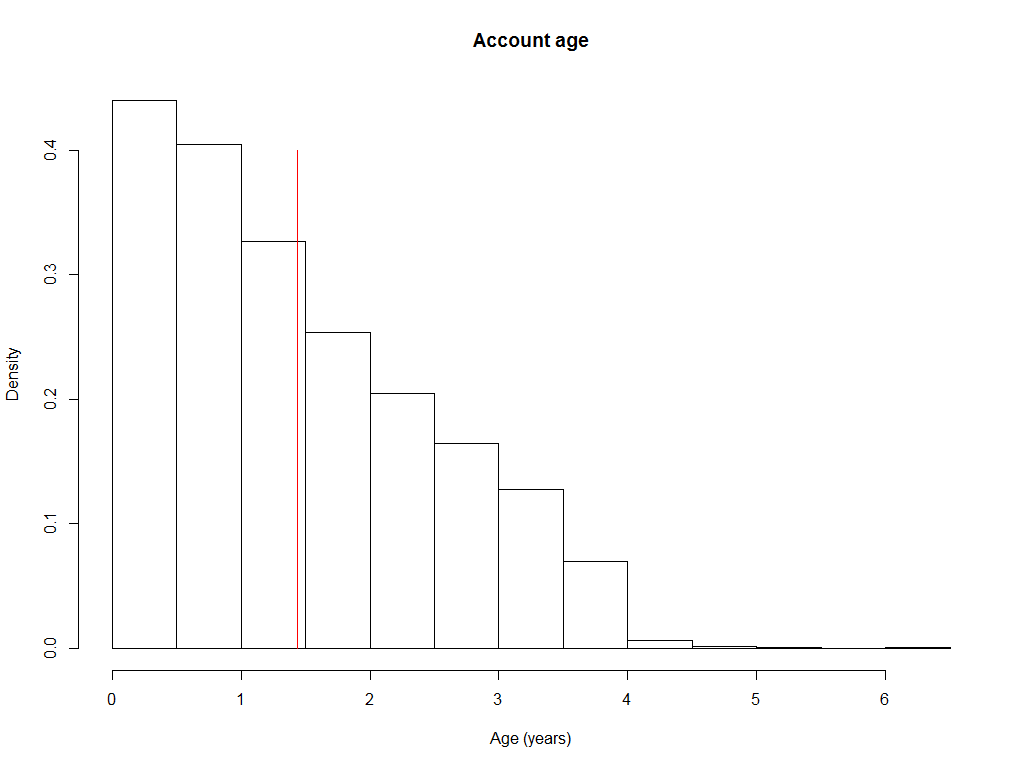
\includegraphics[width=0.8\columnwidth]{figs/account_age_sample5000.png}
\end{center}
\caption{Distribution of account ages. Mean is 1.44 years.}
\label{fig:age}
\end{figure}
 
 We see that 63.2\% of users are registered with language as
 “english”, although as we discuss later, only about half of these
 accounts generate only english tweets. We find users registered under
 31 distinct languages. Second and third most common registered
 languages are Spanish at 12.3\% and Japanese at 4.4\%.

 About 1 in 16000 accounts (9 users in our sample) is ``verified''. Verfied
 accounts are more likely to be the official accounts of well-known
 users like companies and celebrities. The median number of followers
 for these accounts is 3606, versus 1 for the whole population
 (median is 5 if we exclude users with no followers).

 \subsection{Is \id~sampling enough?}

 If Twitter expands the universe of possible \ids~to something much
 larger, such as 64-bit integers, and does not assign \ids~roughly in
 sequence, the \id~space will become very sparse. Facebook expanded
 user \ids~from 32-bit integers
 to potentially-longer alphanumeric strings in 2009 \cite{Minas:2009}.
 In the future, uniform sampling will require other methods of
 discovering user \ids~in an unbiased way. For this reason, we look at
 sampling methods that use the social structure of Twitter.



 \section{Social graph methods}
 \label{sec:graphmethods}

A Twitter user A can be related to another user B by three types of
links:
\begin{itemize}
    \item friend link - A is \emph{following} user B
    \item follower link - A is \emph{followed by} user B
    \item mention - A is \emph{mentioned} in a tweet by B.
\end{itemize}

These links can be used to find other Twitter users starting from a known
Twitter user. We can represent Twitter as a graph, representing users
as vertices, and representing friend or follower links as edges. We
note that this graph is directed and can have up to two edges from
vertex A to B and vice versa. The
Twitter REST API provides calls for gathering connection information
of users. The \api{/user/show} call that returns a user object that includes
fields for friend count and followers count (i.e., the degree of
the vertex). Two calls \api{/followers/ids/}
and \api{/friends/ids} return user \ids~that are followers and friends,
respectively, of the given user (i.e., pointers to the neighbors of
the vertex).

\subsection{Graph traversal}

The most straightforward methods for collecting user \ids~in the social
graph include graph traversal algorithms, such as Breadth-first
search (BFS). One might use such an algorithm to discover all users in the
Twitter social graph; however, because of practical concerns such as
API rate limiting, finding the whole graph is not feasible. Previous
work has shown that breadth-first search is not suitable for sampling
vertices of a graph, as it biases the sample towards vertices of high
degree \cite{Stutzbach:2006, Minas:2009}. This is because vertices
with many edges have a higher probability of being discovered quickly
in a naive graph traversal.

\subsection{Random walks}

Towards generating a sample from the social graph with a desired
distribution, we can turn the social graph into a Markov Chain. Each
vertex becomes a state, and each follower or friend link becomes a
transition. We would like to prove that this chain will converge to a
single stationary distribution. This requires that the chain be
irreducible and ergodic \cite{Upfal:2005}; these properties are
satisfied for random walks on strongly connected finite graphs that
are non-bipartite and have finite transition probabilities. All
reachable vertices in the Twitter graph are strongly connected because
every follower edge has a friend edge in the opposite direction.

A basic random walk that has uniform (inverse degree) transition
probabilities on all edges will result in a stationary distribution
that is biased towards high-degree nodes. Previous work
\cite{Stutzbach:2006, Minas:2009} has shown that in practice random
walks on similar real-world graphs to Twitter do in fact give a skewed
distribution. The Metropolis Hastings algorithm provides a means to
assign transition probabilities to produce a desired stationary
distribution \cite{Upfal:2005}. \cite{Stutzbach:2006} present an
algorithm for a Metropolis Hastings Random Walk (MHRW) on a graph to
produce a uniform stationary distribution. In its essence, the walk
penalizes high degree vertices by making a transition from a lower
degree vertex have a probability proportional to the ratios of the
degrees.

\paragraph{MHRW in Twitter}

We implemented the MHRW for Twitter using the Twitter API. Because the
algorithm works by uniformly randomly proposing one neighbor at a
time, the transition probabilities only must be calculated on proposed
neighbors for sampling, rather than all neighbors. This reduces the
API call cost of each transition in the random walk. The
\api{/user/show} call is relatively inexpensive and is used to get the
degree (friends\_count + followers\_count) of a proposed neighbor, as well
as the user object of an accepted sample. To get the user \id~of the
proposed neighbor, we use the \api{/friends/ids} and \api{/followers/ids} calls.
These calls are heavily rate limited to an average of 1/min and this
dominates the latency of collecting samples. Sampling this way is
about 12x slower than \id~sampling.

Between November 1, 2012 and November 28, 2012, we collected 10 chains
between 10,000 and 80,000 samples in length each. This was a total of
408,184 samples, representing 48,482 unique user accounts.

\subsection{Random walk convergence}

A random walk takes some number of steps before it reaches the
stationary distribution.
With no knowledge of the structure of the graph, we cannot know the
expected time until convergence, and so we rely on visual and
statistical methods for diagnosing convergence.

We rely on scalar estimands to diagnose convergence. These are scalar
properties of the sample, each with its own distribution in the
population. At convergence, the empirical distribution of the scalar
estimand should more closely represent the true distribution than bias
of the starting point. Scalar estimands for Twitter users might
include followers count, friends count, statuses count (number of
tweets), account age, screen name length, and gps coordinates. Factors
that might be used include time zone and registered language.
For this work, we use the first three.

\paragraph{Multiple chains}

The most robust methods for assessing convergence involve comparing
multiple chains. At stationarity, the distribution of each chain
should look the same, with most of the bias from starting points
having dissolved. We pick starting points that are dispersed in the
space of our scalar operands. Specifically we pick users that are far
apart using $L^2$ distance $\sqrt{log(ST_1-ST_2)^2 + log(FR_1-FR_2)^2 +
    log(FO_1-FO_2)^2}$, where $ST$, $FR$, and $FO$ are statuses count,
friends count, and followers count. This method of picking starting
points better ensures that chains mix well
due to shared stationary distribution and not due to starting point.
We collected candidates for starting points rapidly ($>2000/min$) using the
Streaming API.

\paragraph{Visual method: 2D path}

We adopt a method from \cite{Gelman:2003} where multiple chains are
plotted on a pair of axes, one for each of two scalar estimands. The
chains are assumed well-mixed and in their stationary distribution
when the paths intertwine and become indistinguishable. This works
best when the step size within the parameter space is very small as in
Monte Carlo methods for simulating draws from a distribution;
however we applied it to our problem to see if it gave insight.
Figures~\ref{fig:con1},\ref{fig:con2},\ref{fig:con3},
and~\ref{fig:con4} show the progression. ``S'' marks the start point
and diamonds mark the means of the 2nd half of the chains (discussed
in the next method). The means
do not align until many 10's of thousands of iterations.


\begin{figure*}[htb]
    \minipage{0.24\linewidth}
      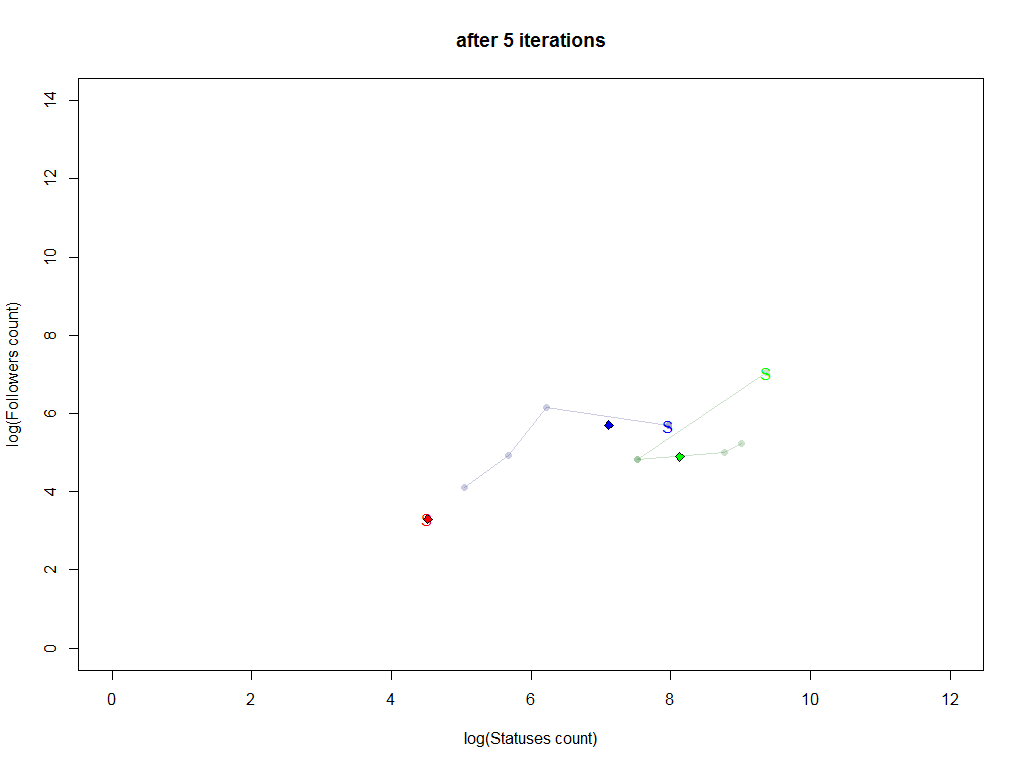
\includegraphics[width=\linewidth]{figs/2dconv_5iters.png}
\caption{}\label{fig:con1}
    \endminipage\hfill
    \minipage{0.24\linewidth}
    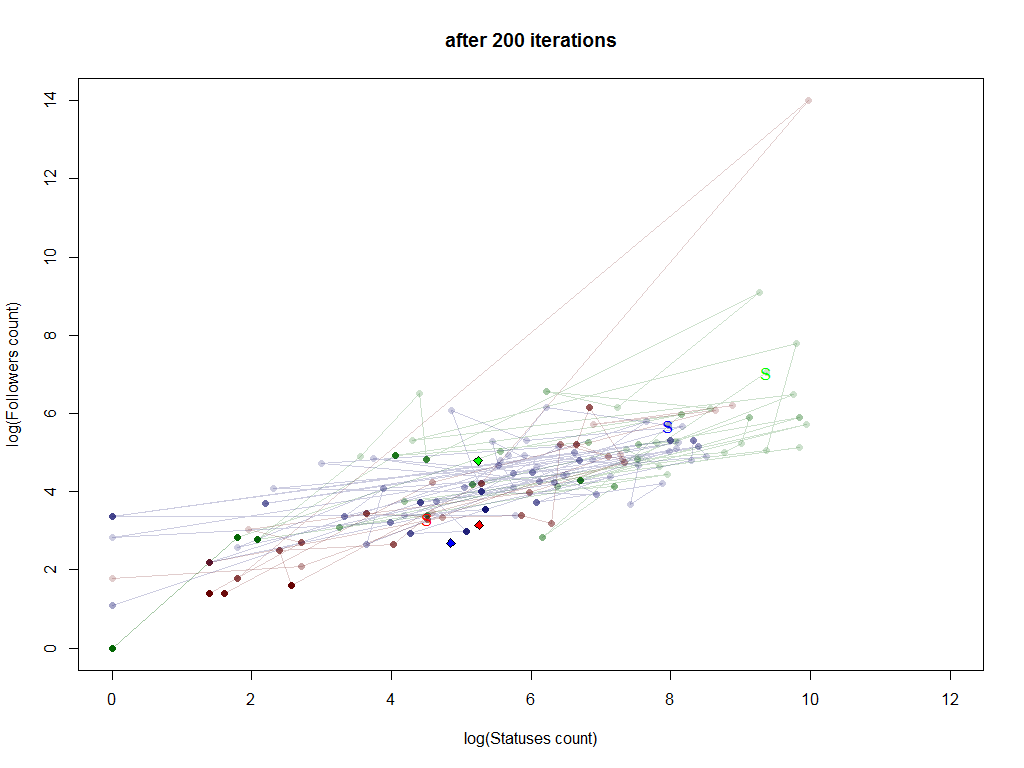
\includegraphics[width=\linewidth]{figs/2dconv_200iters.png}
\caption{}\label{fig:con2}
    \endminipage
    \minipage{0.24\linewidth}
    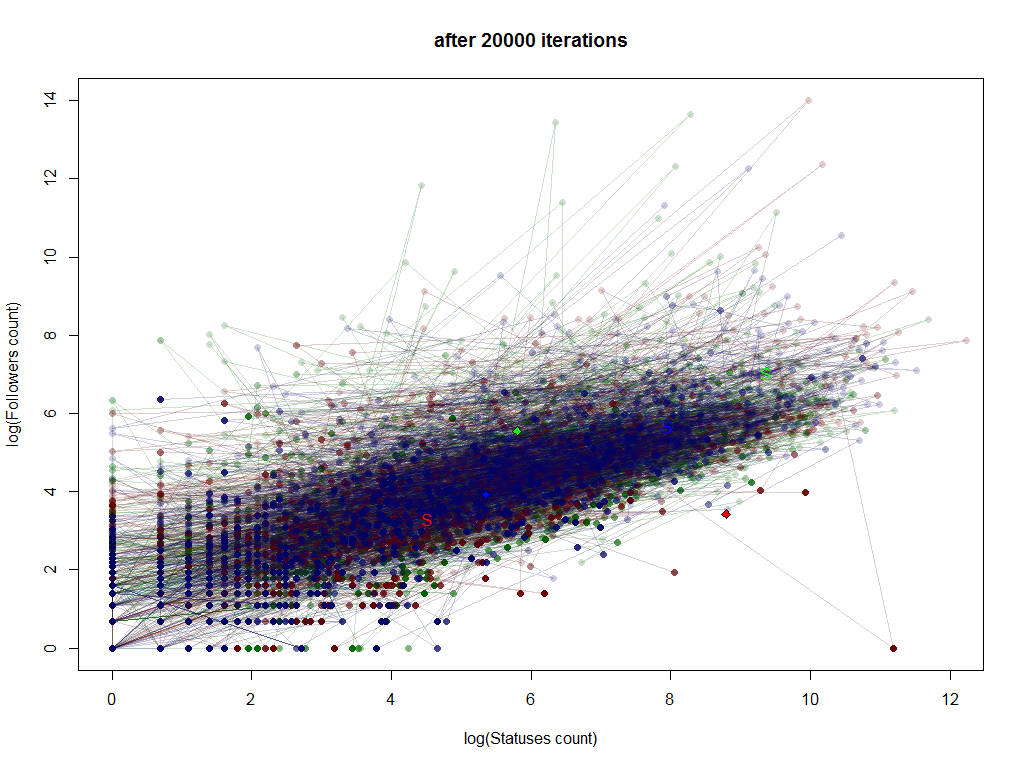
\includegraphics[width=\linewidth]{figs/2dconv_20000iters.png}
\caption{}\label{fig:con3}
    \endminipage\hfill
    \minipage{0.24\linewidth}
    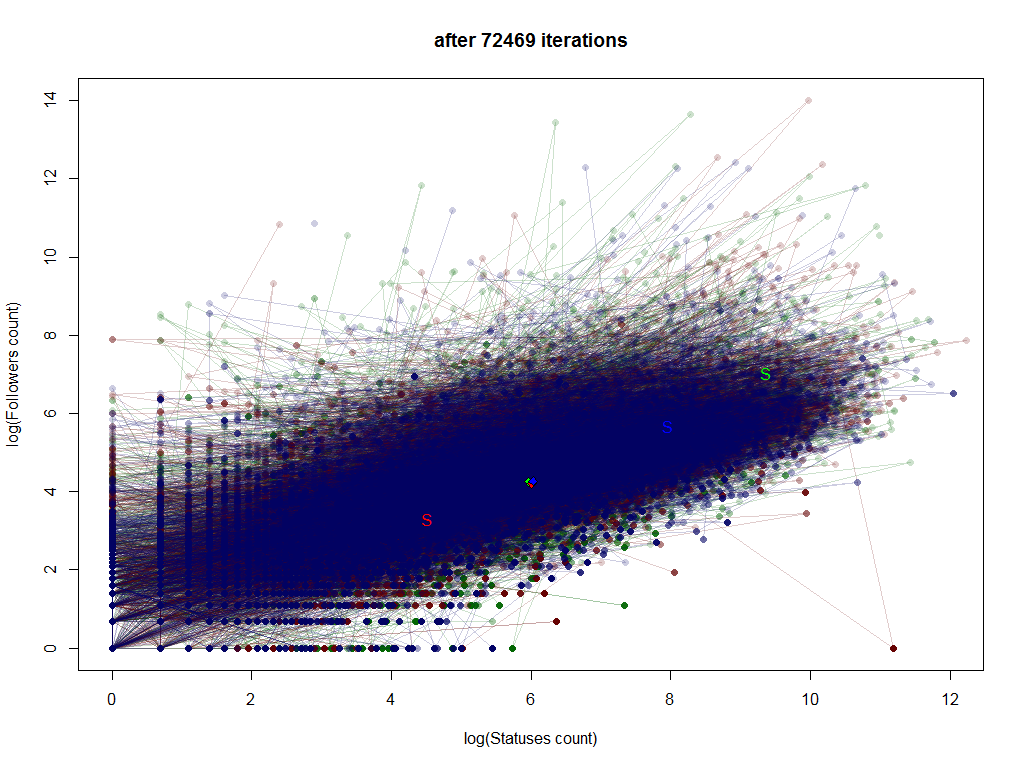
\includegraphics[width=\linewidth]{figs/2dconv_72469iters.png}
\caption{}\label{fig:con4}
    \endminipage
\end{figure*}

\paragraph{Visual method: 2nd half means}

At convergence, the mean of the scalar estimands for the sample should
be the same as that of ground truth or the other chains. It is common
practice to use the 2nd half of a chain to compute the mean.

\begin{figure*}[htb]
    \minipage{0.5\linewidth}
      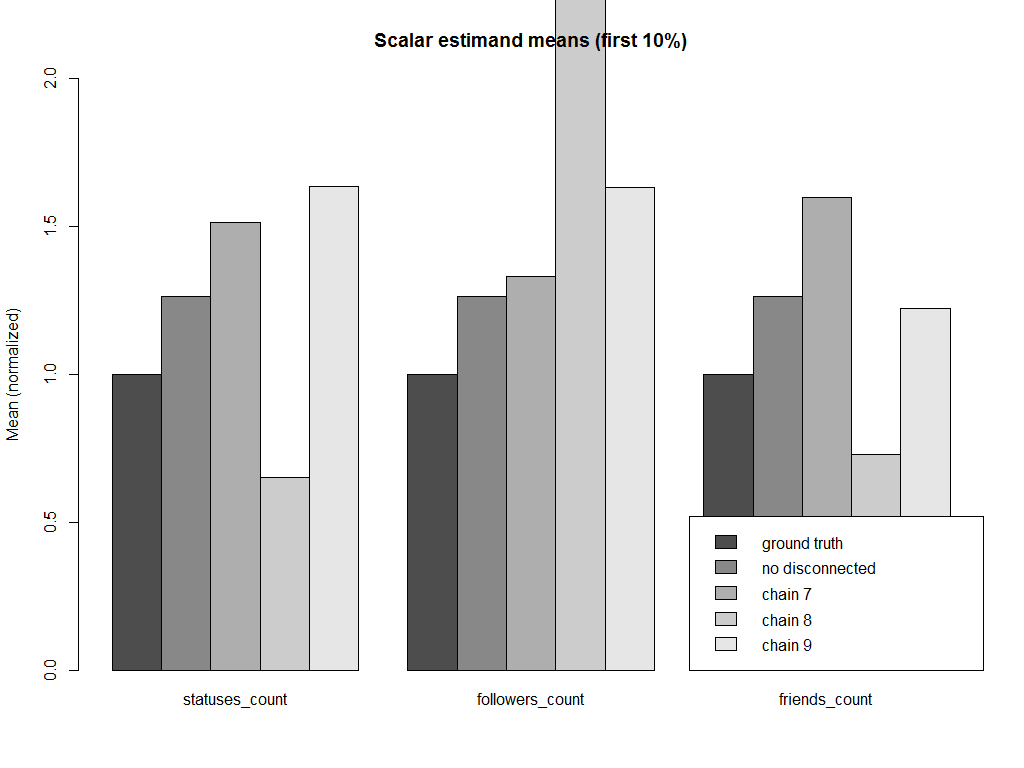
\includegraphics[width=\linewidth]{figs/scalar_estimands_means_10pct.png}
      \caption{Means of scalar estimands for random walks of 70000
          draws and ground
          truth, using first 10\% of the random walk draws.}
\label{fig:means1}
    \endminipage\hfill
    \minipage{0.5\linewidth}
    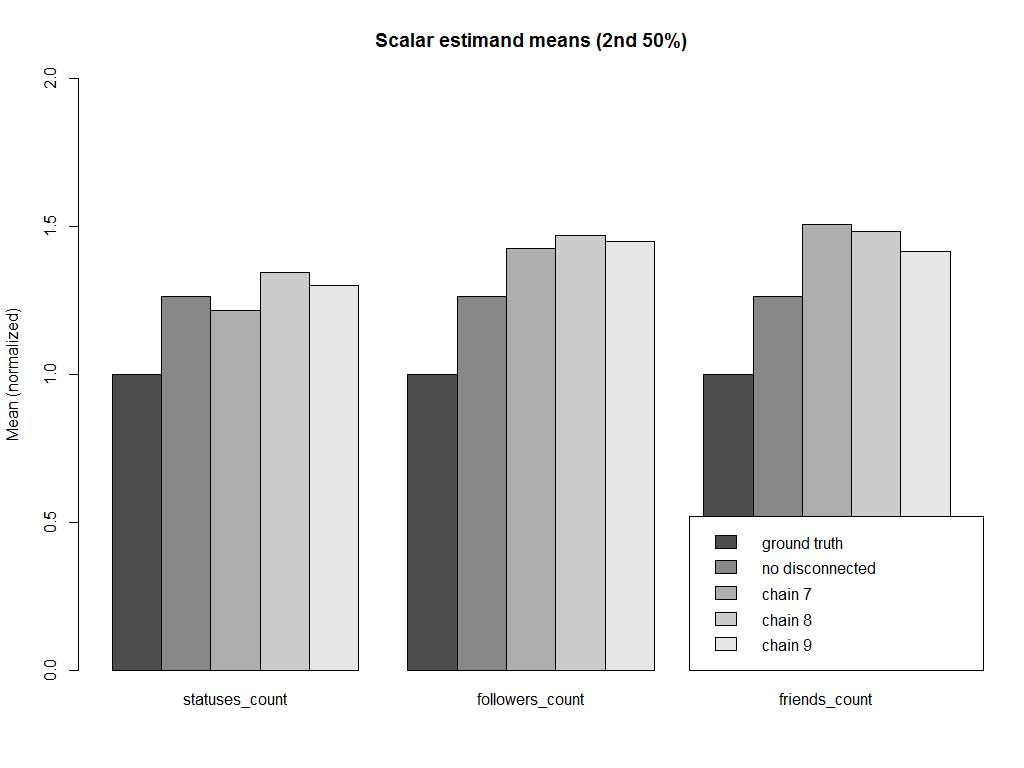
\includegraphics[width=\linewidth]{figs/scalar_estimands_means.png}
    \caption{Means for last 50\% of the random walk draws.}
\label{fig:means2}
    \endminipage
\end{figure*}

The first 10\% (7000) samples have estimand means that vary greatly.
Taking the second half as our sample, the chains' means are close.
Note that the chain means are up to 50\% higher than our ground truth.
This is partly because ground truth sample includes users that are
unreachable in a random walk (i.e. those with zero connections), which
pushes means down. Our sampling frame for random walks is all
connected Twitter users. We reject unconnected samples (20\% of the ground
truth samples) and plot the means as ``not disconnected''. We see that
the chain means for statuses count match this fair comparison.
However, notice that the means of degree count estimands are still
larger. We attribute this to the fact that in practice even the MHRW
will often be biased against vertices with exceptionally low degree
since they are unlikely to be proposed. If one of these vertices was ever
hit, the walk would likely stay in this or other low degree nodes for
a long time, which would bring down the sample mean. If we collected
many more than 70,000 iterations per chain, we could expect the 2nd
half means to converge to those of ``no disconnected''. We find that if
we filter out \id~samples with 1 or fewer connections (30\% of the
samples), the degree means match those of the chains.
Figure~\ref{fig:evolve} shows how the 2nd half mean changes for one of
the chains; the means flatten out at around 50,000 iterations,
providing evidence of possible convergence.

 \begin{figure}[htb]
\begin{center}
    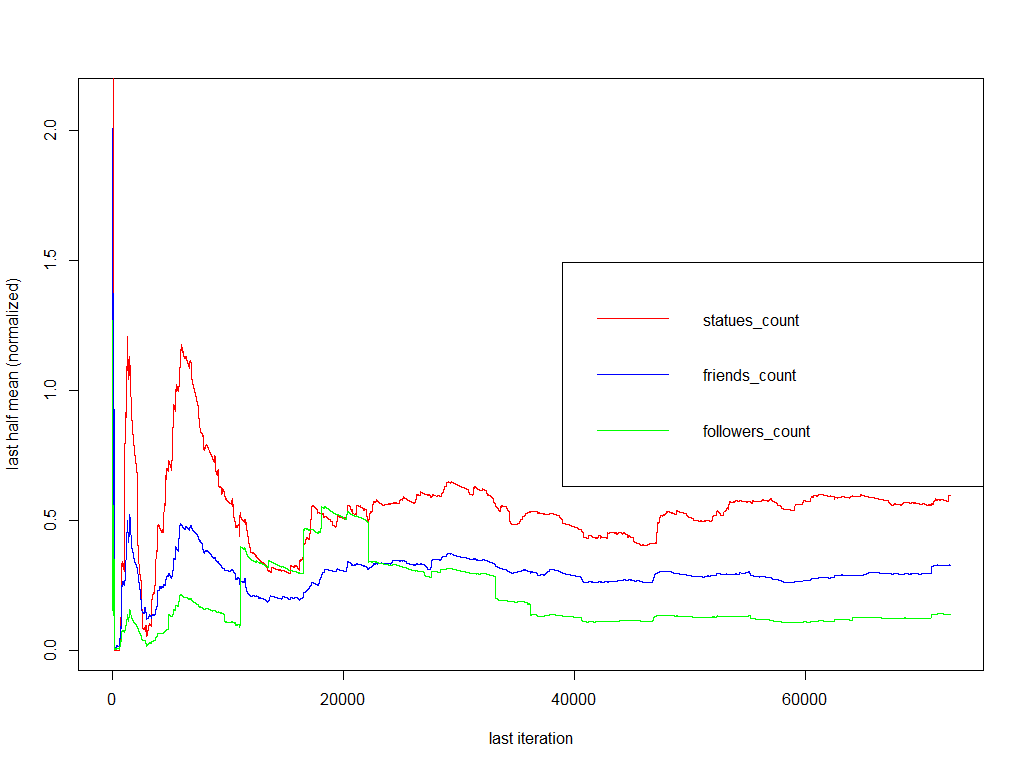
\includegraphics[width=0.8\columnwidth]{figs/stats7_means.png}
\end{center}
\caption{Evolution of 2nd half means as number of iterations grows.}
\label{fig:evolve}
\end{figure}

To assess bias of various sampling methods, \cite{Stutzbach:2006}
looked
at the number of times $X_i$, each node $i$ in the network was sampled. The
distribution of $X_i$'s should be normal with a relatively low variance
of $\frac{num samples}{num nodes}$. For large graphs like Twitter and
under rate limiting, our sample size is far smaller than the graph
size and so we cannot use such methods.

\paragraph{Autocorrelation}

A common practical problem with Markov chain methods is that there is
often correlation between successive draws. This is because taking one
transition may only change parameter values by a small amount. In our
random walk of the Twitter graph, this may be less so since our jumps
through the space of \{status count, friends count, followers count\}
tend to be larger. However, users that are connected or nearby might
conceivably have similar characteristics. In some cases we can use an
autocorrelation diagnostic to suggest whether a chain is well-mixed.
Figure~\ref{fig:autocorr} shows autocorrelation plots for three chains
and the three estimands.

 \begin{figure*}[htb]
\begin{center}
    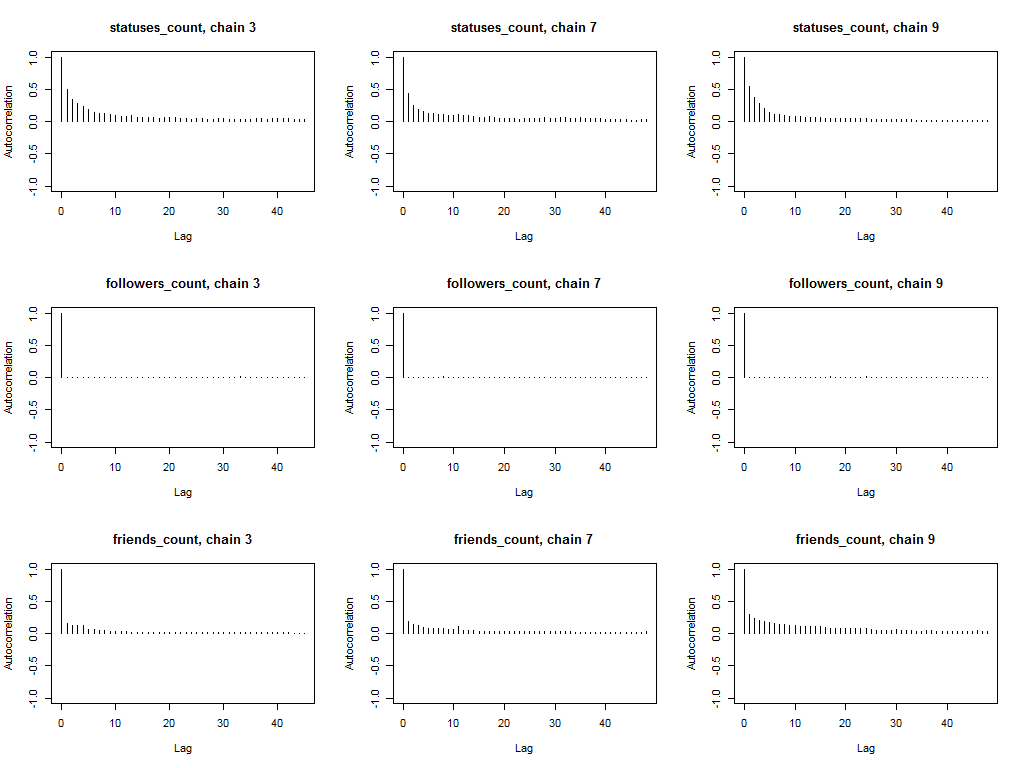
\includegraphics[width=0.8\linewidth]{figs/autocorrelation_chains3-7-9.png}
\end{center}
\caption{Autocorrelation by estimand. Correlation between successive
    draws of Markov chains. As should be the case, the correlation
    drops precipitously as the distance between draws increases.}
\label{fig:autocorr}
\end{figure*}

As should be the case for converged chains, we see that correlation
drops precipitously as distance between draws increases. With our
large jumps this diagnostic likely does not provide a significant
guarentee of convergence, rather just that the chains \emph{might}
have converged.  It does tell us things about the Twitter graph. For
example, statuses count appears somewhat correlated between successive
draws. This could be partly due to staying on one low degree node for
a while but also that neighbors of similar degree tweet at a similar
rate. Also, friends count is more autocorrelated than followers count,
indicating that neighbors tend to have somewhat similar following
behaviors but are not followed similarly. Overall, \emph{behavior} is
correlated between nearby users but \emph{not properties} beyond the
user's direct control.

\paragraph{Convergence diagnostics}

We use the Gelman-Rubin diagnostic from \cite{Gelman:2003} to assess
convergence of multiple chains. This diagnostic uses an estimate of
the marginal posterior variance of a given estimand, comprising a
weighted sum of within- and between-chain variances. Essentially the
diagnostic compares this estimate to the within-chain variance. If a
chain has mixed well, it will have more variability and the
within-chain variance will dominate. The diagnostic is called the
scale-reduction factor or shrink factor, and the higher it is above 1,
the more that adding a greater number of iterations could benefit
convergence.

The Gelman-Rubin diagnostic assumes the estimand has a normal
distribution. Looking at the empirical distributions (not shown for
lack of space) from \id~sampling (with unconnected filtered out), we
see that even under even a log transformation, only the friends count comes
close to resembling a normal distribution. We perform convergence
analysis by computing the diagnostic for increasing numbers of chain
iterations. We calculate the Gelman-Rubin diagnostic for each estimand
using logit or log transforms as needed. Shown in
Figures~\ref{fig:gel-st},\ref{fig:gel-fo}, and~\ref{fig:gel-fr} are
the results for
the three estimands, using 3 chains with up to 72000 iterations each.  

\begin{figure*}[htb]
    \minipage{0.32\linewidth}
      \includegraphics[width=\linewidth]{figs/gelman_all/gelman_statuses_count_3chains_70000iters.png}
      \caption{Gelman-Rubin diagnostic for increasing iterations.
          Chains are said to converge when the diagnostic settles
          close to 1.}
\label{fig:gel-st}
    \endminipage\hfill
    \minipage{0.32\linewidth}
      \includegraphics[width=\linewidth]{figs/gelman_all/gelman_followers_count_3chains_70000iters.png}
    \caption{}
\label{fig:gel-fo}
    \endminipage
    \minipage{0.32\linewidth}
      \includegraphics[width=\linewidth]{figs/gelman_all/gelman_friends_count_3chains_70000iters.png}
      \caption{}
\label{fig:gel-fr}
    \endminipage\hfill
\end{figure*}

We see that all estimands appear to converge by around 52000
iterations.

\paragraph{Distribution tests}

When parallel chains have converged, their distributions of the scalar
estimands should be very similar. Because our scalar estimands have
non-normal distributions, we considered the non-parametric two-sample
Kolmogorov-Smirnov test between the 2nd halves of pairs of chains. The
KS test assumes continuous distributions (i.e., no ties). Since all of our
estimands are integer-valued, we jittered the samples with normal
distributions to satisfy this
constraint. 
The result was that these tests always rejected the null hypothesis
(no difference between the distributions) with very low p-value. The
test may be far too sensitive for \emph{practical} use in our problem.

